\documentclass[12pt, t, aspectratio=169]{beamer}
\usepackage{ctex}
\usepackage{graphicx}
\usepackage{amsmath}
\usepackage{amssymb}
\usepackage{hyperref}
\usepackage{tikz}
\usetikzlibrary{positioning}

% 设置主题与配色
\usetheme{Madrid}
\usecolortheme{default}
\setbeamertemplate{navigation symbols}{} % 去除导航符号

% 标题页信息
\title{第一章：深度学习革命 - 开启智能新纪元}
% \institute{}
\author{《深度学习基础》课程小组}
\date{\today}

\begin{document}

% 标题页
\begin{frame}
    \titlepage
\end{frame}

% 目录页
\begin{frame}
    \frametitle{目录}
    \tableofcontents
\end{frame}

% 第零部分：深度学习知识图谱
\section{深度学习的知识图谱}
\begin{frame}
    % \frametitle{深度学习知识图谱}

    \begin{center}
    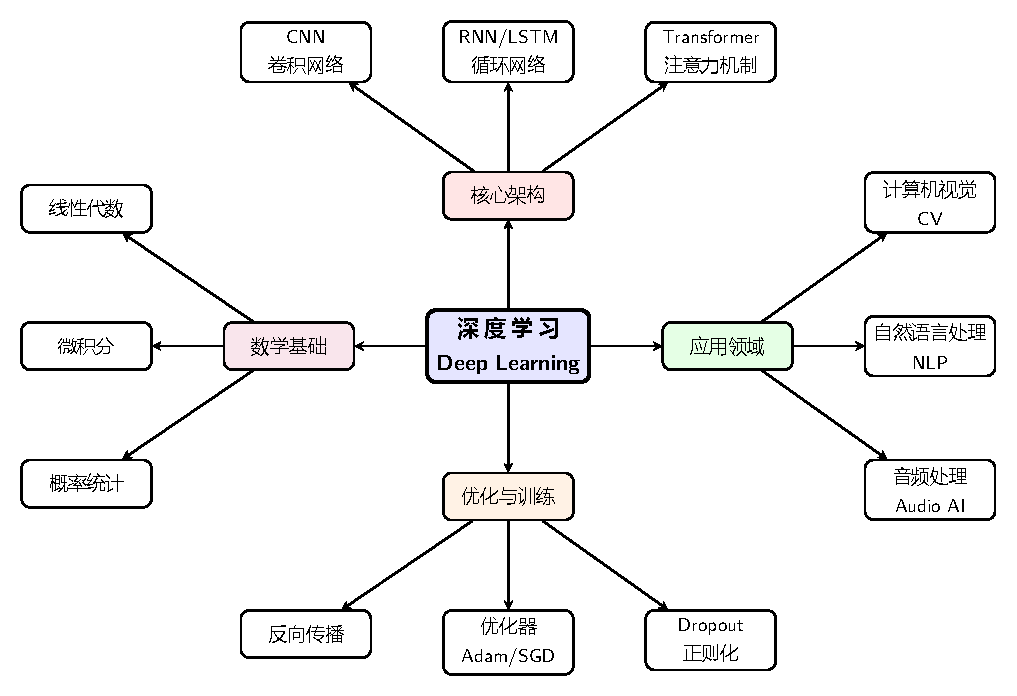
\includegraphics[width=0.7\textwidth]{ch01-graph-v2.pdf}
    \end{center}

\end{frame}

%%%%%%%%%%%%%%%%%%%%%%%%%%%%%%%%%%%%%%%%%%%%%%%%%%%%%%%%%%%%%%%%%%%%%%%%%%
% 第零部分：深度学习的概念与发展历程
\section{深度学习的概念与发展历程}

\begin{frame}
    \frametitle{深度学习是什么？}
    \begin{itemize}
    \item 深度学习是机器学习的一个子领域，思路来源于人脑的神经网络结构。
    \item 它通过构建包含多个隐藏层的深层网络，能够自动从数据中学习特征表示。
    \item 无需人工手动设计特征，利用海量数据端到端地优化模型参数。
    \item 反向传播算法和强大的算力是其能够训练超大规模模型的关键技术支撑。
    \item 在计算机视觉、自然语言处理和语音识别等领域超越了人类水平。
    \item 作为当前人工智能发展的主要驱动力，正深刻改变着各行各业的生产方式。
    \end{itemize}
\end{frame}

% \begin{frame}
%     \frametitle{深度学习的发展历程}
%     \begin{enumerate}
%     \item \textbf{1943年}：Warren McCulloch 和 Walter Pitts 提出首个\textbf{人工神经元模型} (M-P模型)，奠定理论基础。
%     \item \textbf{1958年}：Frank Rosenblatt 发明\textbf{感知器} (Perceptron)，实现了最早的机器学习算法。
%     \item \textbf{1986年}：Geoffrey Hinton 等人重新发现并推广\textbf{反向传播算法} (Backpropagation)，解决了多层网络训练难题。
%     \item \textbf{2012年}：\textbf{AlexNet} 在 ImageNet 竞赛中以压倒性优势夺冠，标志\textbf{深度学习时代}正式到来。
%     \item \textbf{2017年}：Google 提出 \textbf{Transformer} 架构 (“Attention is All You Need”)，彻底变革自然语言处理领域。
%     \item \textbf{2022年}：OpenAI 发布 \textbf{ChatGPT}，基于大语言模型 (LLM) 的生成式 AI 引发全球热潮。
%     \end{enumerate}
% \end{frame}

% \begin{frame}{深度学习的发展历程：关键突破与问题解决}
%     \begin{enumerate}
%         \item \textbf{1943 年 (M-P 模型)} $\rightarrow$ 解决了“如何用数学模拟生物神经元”的理论建模问题。
%         \item \textbf{1958 年 (感知器)} $\rightarrow$ 解决了**“机器如何从数据中自动学习分类”**的算法实现问题。
%         \item \textbf{1986 年 (反向传播)} $\rightarrow$ 解决了**“多层神经网络无法有效训练”**的梯度更新难题。
%         \item \textbf{2012 年 (AlexNet)} $\rightarrow$ 解决了**“传统方法在复杂图像识别中精度瓶颈”**的问题，验证了深度架构威力。
%         \item \textbf{2017 年 (Transformer)} $\rightarrow$ 解决了**“RNN 无法并行计算及长距离依赖丢失”**的效率与性能问题。
%         \item \textbf{2022 年 (ChatGPT)} $\rightarrow$ 解决了**“AI 缺乏通用理解与人类对齐交互”**的能力，开启生成式 AI 时代。
%     \end{enumerate}
% \end{frame}

\begin{frame}{深度学习发展历程：关键突破}
    \centering
    \renewcommand{\arraystretch}{1.5} % 增加行高，使表格更疏朗
    \begin{tabular}{|c|l|l|}
        \hline
        \textbf{年份} & \textbf{核心突破} & \textbf{解决的关键问题} \\
        \hline
        1943 & M-P 神经元模型 & 提出神经元的数学形式化描述 \\
        \hline
        1958 & 感知器 (Perceptron) & 实现首个可训练的线性分类算法 \\
        \hline
        1986 & 反向传播 (BP) & 解决多层网络权重无法有效更新的难题 \\
        \hline
        2012 & AlexNet & 突破图像识别精度瓶颈，验证深度架构威力 \\
        \hline
        2017 & Transformer & 解决序列建模无法并行及长依赖丢失问题 \\
        \hline
        2022 & ChatGPT (LLM) & 实现通用语言理解与人类意图对齐 \\
        \hline
    \end{tabular}
\end{frame}

%%%%%%%%%%%%%%%%%%%%%%%%%%%%%%%%%%%%%%%%%%%%%%%%%%%%%%%%
% 第一部分：深度学习的数学基础
\section{深度学习的数学基础}

\begin{frame}{数学基础：微积分 (Calculus)}
    \framesubtitle{优化的引擎：如何更新参数？}
    \begin{enumerate}
        \item \textbf{导数与偏导数}：计算损失函数对每个权重的变化率，指示调整方向。
        \item \textbf{梯度 (Gradient)}：由偏导数组成的向量，指向损失函数增长最快的方向。
        \item \textbf{链式法则 (Chain Rule)}：反向传播的核心，用于计算深层网络中复合函数的导数。
        \item \textbf{泰勒展开}：用于近似损失函数曲面，推导牛顿法等二阶优化算法。
        \item \textbf{积分}：在连续概率分布及计算期望值（如损失函数的期望）时使用。
        \item \textbf{核心作用}：没有微积分，就无法通过梯度下降法自动训练神经网络。
    \end{enumerate}
\end{frame}

\begin{frame}{数学基础：线性代数 (Linear Algebra)}
    \framesubtitle{数据的语言：如何高效表示与计算？}
    \begin{enumerate}
        \item \textbf{张量 (Tensors)}：多维数组，是存储图像、文本嵌入及网络参数的基本数据结构。
        \item \textbf{矩阵乘法}：神经网络前向传播的核心运算，实现输入与权重的线性变换。
        \item \textbf{特征值与特征向量}：用于分析矩阵性质，在 PCA 降维及理解 RNN 稳定性中至关重要。
        \item \textbf{矩阵分解}：如 SVD 分解，用于模型压缩、推荐系统及初始化策略。
        \item \textbf{向量空间}：词嵌入 (Word Embeddings) 将语义映射为向量，通过距离衡量相似度。
        \item \textbf{核心作用}：利用 GPU 并行加速矩阵运算，是深度学习高效计算的基石。
    \end{enumerate}
\end{frame}

\begin{frame}{数学基础：概率统计 (Probability \& Statistics)}
    \framesubtitle{不确定性的建模：如何处理噪声与推断？}
    \begin{enumerate}
        \item \textbf{概率分布}：建模数据生成过程（如高斯分布），用于生成模型 (VAE, Diffusion)。
        \item \textbf{贝叶斯定理}：用于先验知识融合及不确定性估计，是朴素贝叶斯及贝叶斯深度学习的基础。
        \item \textbf{最大似然估计 (MLE)}：推导损失函数（如交叉熵）的理论依据，用于参数优化。
        \item \textbf{期望与方差}：衡量模型预测的准确性与稳定性，用于 Batch Normalization 等技巧。
        \item \textbf{采样技术}：如 MCMC 或随机梯度下降中的 Mini-batch 采样，用于近似计算。
        \item \textbf{核心作用}：处理数据噪声、评估模型置信度及构建生成式 AI 的核心理论。
    \end{enumerate}
\end{frame}

%%%%%%%%%%%%%%%%%%%%%%%%%%%%%%%%%%%%%%%%%%%%%%%%%%%%%%%%
% 第二部分：深度学习的优化与训练
\section{深度学习的优化与训练}

\begin{frame}
    \frametitle{反向传播算法 (Backpropagation)}
    \framesubtitle{核心：链式法则 (Chain Rule)}
    
    \textbf{核心思想}：将误差从输出层向输入层逐层传递，计算每个参数对总损失的贡献。
    
    \begin{enumerate}
        \item \textbf{前向传播}：$x \rightarrow \dots \rightarrow \hat{y}$，计算预测值。
        \item \textbf{计算损失}：$L = \text{Loss}(\hat{y}, y)$，衡量误差。
        \item \textbf{反向求导}：利用链式法则 $\frac{\partial L}{\partial w} = \frac{\partial L}{\partial \hat{y}} \cdot \frac{\partial \hat{y}}{\partial z} \cdot \frac{\partial z}{\partial w}$。
        \item \textbf{更新参数}：$w_{new} = w_{old} - \eta \cdot \frac{\partial L}{\partial w}$。
    \end{enumerate}
    
    \begin{alertblock}{关键点}
        反向传播使得深层网络中每一层的权重都能根据最终误差进行有效调整，是训练深度网络的基石。
    \end{alertblock}
\end{frame}

\begin{frame}
    \frametitle{主流优化器 (Optimizers)}
    \framesubtitle{如何更聪明地更新权重？}
    
    \begin{columns}[T]
        \column{0.48\textwidth}
        \textbf{SGD (随机梯度下降)}
        \begin{itemize}
            \item 基础版本，仅依赖当前梯度。
            \item 容易陷入局部最优或震荡。
            \item 需仔细调整学习率。
        \end{itemize}
        
        \vspace{0.3cm}
        \textbf{Momentum (动量法)}
        \begin{itemize}
            \item 引入“惯性”，积累之前的梯度方向。
            \item 加速收敛，抑制震荡。
        \end{itemize}
        
        \column{0.48\textwidth}
        \textbf{Adam (自适应矩估计)} \textcolor{red}{\textbf{(最常用)}}
        \begin{itemize}
            \item 结合 Momentum + RMSProp。
            \item 为每个参数自适应调整学习率。
            \item 收敛快，对超参数不敏感。
        \end{itemize}
        
        \vspace{0.3cm}
        \textbf{其他变种}
        \begin{itemize}
            \item AdaGrad, RMSprop, AdamW (解决权重衰减问题)。
        \end{itemize}
    \end{columns}
    
\end{frame}

\begin{frame}
    \frametitle{正则化技术 (Regularization)}
    \framesubtitle{防止过拟合 (Overfitting)}
    
    \textbf{什么是过拟合？} 模型在训练集表现完美，但在测试集表现糟糕（死记硬背）。
    
    \vspace{0.3cm}
    \begin{itemize}
        \item \textbf{L1 / L2 正则化}
        \begin{itemize}
            \item 在损失函数中加入权重的惩罚项 ($\lambda \|w\|$)。
            \item L1 倾向于产生稀疏权重，L2 倾向于小权重。
        \end{itemize}
        
        % \vspace{0.3cm}
        \item \textbf{Dropout} \textcolor{blue}{\textbf{(深度学习标配)}}
        \begin{itemize}
            \item 训练时随机“丢弃”一部分神经元（置为0）。
            \item 强迫网络不依赖特定路径，增强鲁棒性。
            \item 测试时恢复所有神经元，权重按比例缩放。
        \end{itemize}
        
        % \vspace{0.3cm}
        \item \textbf{早停法 (Early Stopping)}
        \begin{itemize}
            \item 当验证集误差不再下降时，提前停止训练。
        \end{itemize}
    \end{itemize}
\end{frame}

\begin{frame}
    \frametitle{其他关键训练技巧}
    \framesubtitle{让模型训练更稳定、更快}
    
    \begin{enumerate}
        \item \textbf{批量归一化 (Batch Normalization, BN)}
        \begin{itemize}
            \item 将每层输入强制拉回到均值0、方差1的分布。
            \item 允许使用更大的学习率，加速收敛，减少对初始化的敏感。
        \end{itemize}
        
        % \vspace{0.3cm}
        \item \textbf{学习率调度 (Learning Rate Scheduling)}
        \begin{itemize}
            \item 动态调整学习率（如：随epoch增加而衰减，或热身 Warmup）。
            \item 避免初期震荡过大或后期无法收敛到最优。
        \end{itemize}
        
        % \vspace{0.3cm}
        \item \textbf{数据增强 (Data Augmentation)}
        \begin{itemize}
            \item 通过旋转、裁剪、噪声等手段扩充训练数据。
            \item 提升模型泛化能力，特别是CV领域。
        \end{itemize}
        
        % \vspace{0.3cm}
        \item \textbf{迁移学习 (Transfer Learning)}
        \begin{itemize}
            \item 加载在大规模数据集（如ImageNet）上预训练的权重。
            \item 在小数据集上微调 (Fine-tuning)，省时省力效果好。
        \end{itemize}
    \end{enumerate}
\end{frame}

%%%%%%%%%%%%%%%%%%%%%%%%%%%%%%%%%%%%%%%%%%%%%%%%%%%%%%%%%%%%%%%%%
% 第三部分：核心架构
\section{深度学习的核心架构}

% --- CNN ---
\begin{frame}
    \frametitle{卷积神经网络 (CNN)}
    \framesubtitle{计算机视觉的基石}
    
    \begin{itemize}
        \item \textbf{核心思想}：模拟生物视觉皮层，通过局部感知和权值共享提取特征。
        \item \textbf{关键组件}：
        \begin{itemize}
            \item \textbf{卷积层}：提取边缘、纹理等局部特征。
            \item \textbf{池化层}：降维，保留主要特征，提高平移不变性。
            \item \textbf{全连接层}：整合特征进行分类。
        \end{itemize}
        \item \textbf{主要优势}：参数效率高，擅长处理网格状数据（如图像）。
        \item \textbf{典型应用}：图像分类 (ResNet)、目标检测 (YOLO)、人脸识别。
    \end{itemize}
    
    \begin{block}{代表模型}
        LeNet-5, AlexNet, VGG, ResNet, EfficientNet
    \end{block}
\end{frame}

% --- RNN ---
\begin{frame}
    \frametitle{循环神经网络 (RNN)}
    \framesubtitle{处理序列数据的先驱}
    
    \begin{itemize}
        \item \textbf{核心思想}：引入“记忆”单元，当前输出不仅取决于当前输入，还取决于上一时刻的状态。
        \item \textbf{工作机制}：具有循环连接，信息在时间步之间传递，形成内部状态。
        \item \textbf{主要优势}：天然适合处理变长序列数据（如文本、时间序列）。
        \item \textbf{局限性}：难以捕捉长距离依赖，容易出现梯度消失或爆炸问题。
        \item \textbf{典型应用}：语言建模、简单的时间序列预测。
    \end{itemize}
    
    \begin{alertblock}{注意}
        标准 RNN 在实际应用中常被 LSTM 或 GRU 取代，以解决长依赖问题。
    \end{alertblock}
\end{frame}

% --- LSTM ---
\begin{frame}
    \frametitle{长短期记忆网络 (LSTM)}
    \framesubtitle{解决长距离依赖的专家}
    
    \begin{itemize}
        \item \textbf{核心改进}：引入复杂的“门控机制”来控制信息的流动和遗忘。
        \item \textbf{三大 gates}：
        \begin{itemize}
            \item \textbf{遗忘门}：决定丢弃哪些旧信息。
            \item \textbf{输入门}：决定更新哪些新信息。
            \item \textbf{输出门}：决定基于当前状态输出什么。
        \end{itemize}
        \item \textbf{主要优势}：有效缓解梯度消失，能捕捉长序列中的长期依赖关系。
        \item \textbf{典型应用}：机器翻译、语音识别、股票价格预测、文本生成。
    \end{itemize}
    
    \begin{block}{变体}
        GRU (Gated Recurrent Unit)：LSTM 的简化版，参数更少，训练更快。
    \end{block}
\end{frame}

% --- GAN ---
\begin{frame}
    \frametitle{生成对抗网络 (GAN)}
    \framesubtitle{生成式学习的博弈论}
    
    \begin{itemize}
        \item \textbf{核心思想}：基于博弈论，由两个网络相互对抗进行训练。
        \item \textbf{双网络结构}：
        \begin{itemize}
            \item \textbf{生成器 (Generator)}：制造假数据，试图欺骗判别器。
            \item \textbf{判别器 (Discriminator)}：分辨真假数据，试图识破生成器。
        \end{itemize}
        \item \textbf{训练目标}：达到纳什均衡，使生成器能产生以假乱真的数据。
        \item \textbf{典型应用}：超分辨率重建、风格迁移、人脸生成、数据增强。
    \end{itemize}
    
    \begin{alertblock}{挑战}
        训练不稳定，容易出现模式崩溃 (Mode Collapse) 问题。
    \end{alertblock}
\end{frame}

% --- Transformer ---
\begin{frame}
    \frametitle{Transformer (注意力机制)}
    \framesubtitle{当今大模型的核心架构}
    
    \begin{itemize}
        \item \textbf{核心思想}：完全摒弃循环和卷积，仅依靠\textbf{自注意力机制 (Self-Attention)}。
        \item \textbf{关键机制}：
        \begin{itemize}
            \item \textbf{注意力}：直接计算序列中任意两个位置的相关性，无论距离多远。
            \item \textbf{并行计算}：所有位置同时处理，训练速度远超 RNN/LSTM。
            \item \textbf{位置编码}：注入序列顺序信息。
        \end{itemize}
        \item \textbf{主要优势}：极强的长距离建模能力，易于并行化，扩展性极佳。
        \item \textbf{典型应用}：大语言模型 (LLM), 机器翻译 (BERT, GPT 系列), 视觉 Transformer (ViT)。
    \end{itemize}
    
    \begin{block}{历史地位}
        论文 "Attention is All You Need" (2017) 开启了现代 AI 的大模型时代。
    \end{block}
\end{frame}

%%%%%%%%%%%%%%%%%%%%%%%%%%%%%%%%%%%%%%%%%%%%%%%%%%%%%%%%%%%%%%%%%
% 第四部分：应用与展望
\section{深度学习的应用与展望}

\begin{frame}{深度学习在计算机视觉领域的应用}
    \begin{enumerate}
        \item \textbf{图像分类}：识别图片中的主要物体类别 (如 ResNet, EfficientNet)。
        \item \textbf{目标检测}：定位并识别图中多个物体的位置 (如 YOLO, Faster R-CNN)。
        \item \textbf{图像分割}：像素级区分物体轮廓，用于医疗影像分析。
        \item \textbf{人脸识别}：用于身份验证、门禁系统及手机解锁。
        \item \textbf{图像生成}：根据文字描述生成逼真图像 (如 Stable Diffusion, Midjourney)。
        \item \textbf{视频分析}：动作识别、行为监控及自动驾驶环境感知。
    \end{enumerate}
\end{frame}

\begin{frame}{深度学习在自然语言处理领域的应用}
    \begin{enumerate}
        \item \textbf{机器翻译}：实现高质量的多语言互译 (如 Google Translate, DeepL)。
        \item \textbf{大语言模型 (LLM)}：智能对话、内容创作与代码生成 (如 ChatGPT)。
        \item \textbf{情感分析}：自动判断文本的情感倾向 (正面/负面/中立)。
        \item \textbf{文本摘要}：从长篇文章中自动提取核心观点生成简报。
        \item \textbf{命名实体识别}：自动抽取人名、地名、机构名等关键信息。
        \item \textbf{智能问答}：基于知识库或文档自动回答用户提出的问题。
    \end{enumerate}
\end{frame}

\begin{frame}{深度学习在音频处理领域的应用}
    \begin{enumerate}
        \item \textbf{语音识别 (ASR)}：将语音实时转换为文本 (如 Whisper)。
        \item \textbf{语音合成 (TTS)}：生成逼真的人声和情感语音 (如 VITS)。
        \item \textbf{声音分离}：从混合音频中分离人声或特定乐器。
        \item \textbf{音频增强}：智能降噪、回声消除及音质修复。
        \item \textbf{音乐生成}：根据文本描述自动创作音乐和音效 (如 Suno)。
        \item \textbf{声纹识别}：通过声音特征进行身份验证和安全监控。
    \end{enumerate}
\end{frame}

\begin{frame}{深度学习在其他领域的应用}
    \begin{enumerate}
        \item \textbf{推荐系统}：电商与流媒体平台的个性化内容精准推送 (如 TikTok, Netflix)。
        \item \textbf{生物医疗}：蛋白质结构预测 (AlphaFold) 及新药分子筛选与设计。
        \item \textbf{金融科技}：高频交易策略、信用评分及欺诈检测与风险控制。
        \item \textbf{自动驾驶}：多传感器融合感知、路径规划及车辆决策控制。
        \item \textbf{科学计算}：加速气象预报、流体力学模拟及材料科学发现。
        \item \textbf{工业制造}：生产线缺陷检测、设备故障预测性维护及机器人控制。
    \end{enumerate}
\end{frame}

\begin{frame}{深度学习的未来发展趋势}
    \begin{enumerate}
        \item \textbf{通向通用人工智能 (AGI)}：\\ 从专用弱 AI 向具备通用推理、规划及世界模型能力的强 AI 演进。
        \item \textbf{多模态融合 (Multimodal)}：\\ 打破文本、图像、音频界限，实现像人类一样的全方位感知与理解。
        \item \textbf{可解释性与安全 (XAI \& Safety)}：\\ 打开“黑盒”，确保模型决策透明、可控，解决伦理对齐与幻觉问题。
        \item \textbf{高效能与绿色 AI}：\\ 发展模型压缩、量化及稀疏化技术，降低算力消耗，实现端侧部署。
        \item \textbf{数据效率与小样本学习}：\\ 减少对海量标注数据的依赖，提升少样本 (Few-shot) 及自监督学习能力。
        \item \textbf{神经符号结合 (Neuro-Symbolic)}：\\ 融合深度学习的感知力与符号逻辑的推理力，实现更严谨的逻辑推断。
    \end{enumerate}
\end{frame}

%%%%%%%%%%%%%%%%%%%%%%%%%%%%%%%%%%%%%%%%%%%%%%%%%%%%%%%%%%%%%%%%%%%%%%%%%%%
\section{人工智能、世界模型的知识图谱}
\begin{frame}
    % \frametitle{人工智能的知识图谱}
    \begin{center}
    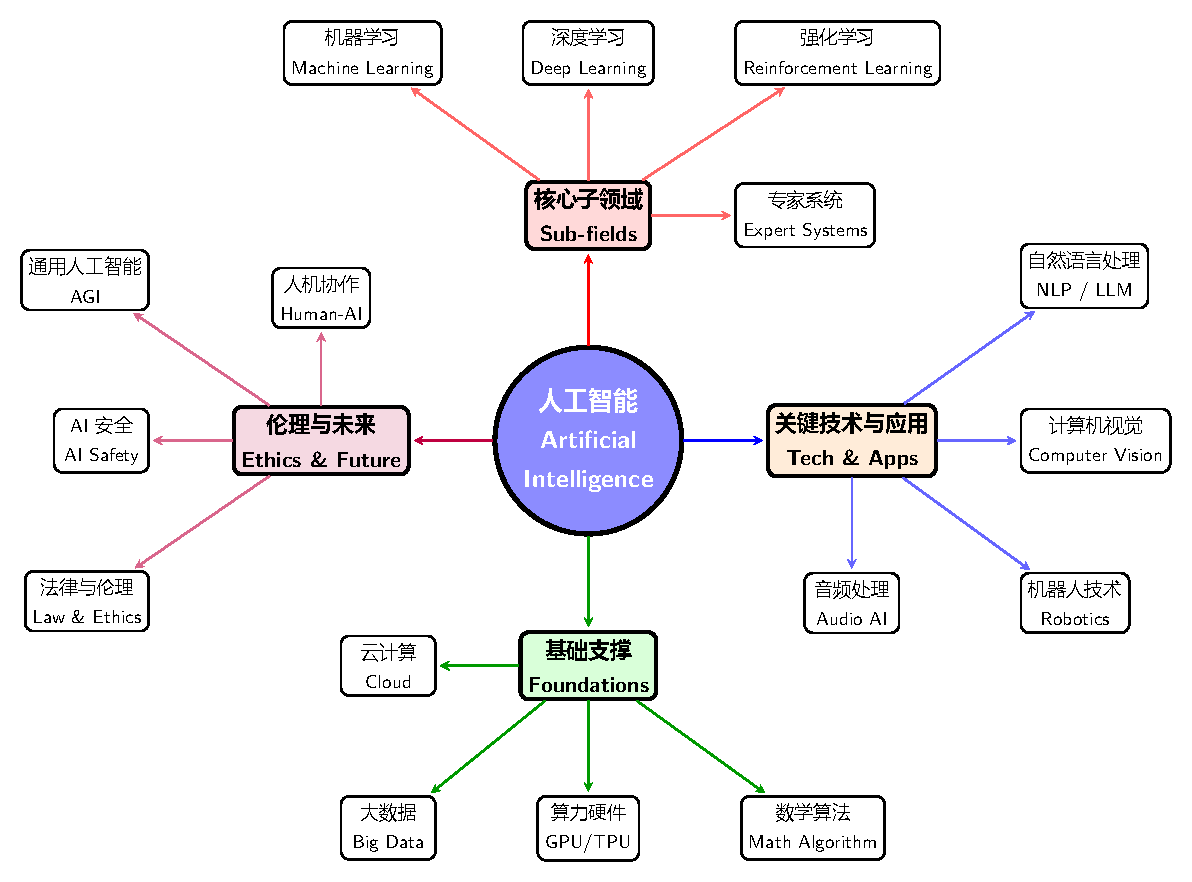
\includegraphics[width=0.7\textwidth]{ch01-graph-v3.pdf}
    \end{center}
\end{frame}

\begin{frame}
    % \frametitle{世界模型的知识图谱}
    \begin{center}
    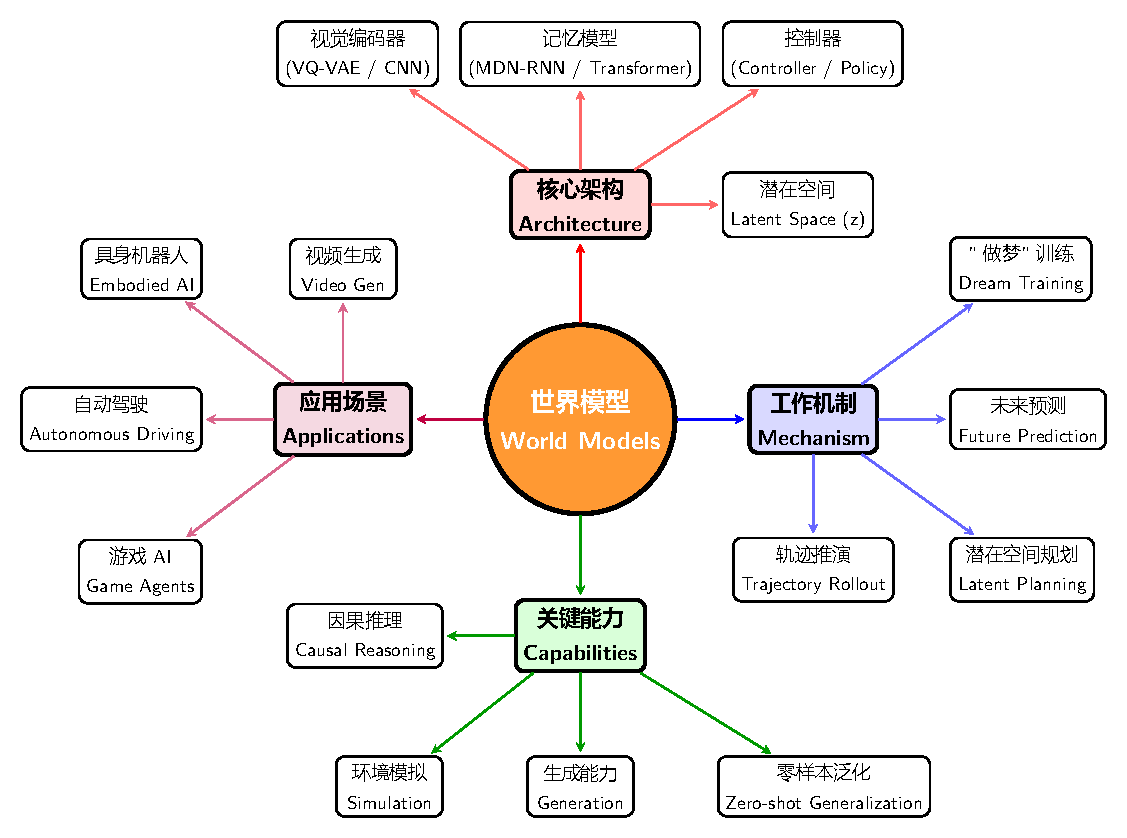
\includegraphics[width=0.7\textwidth]{ch01-graph-v4.pdf}
    \end{center}
\end{frame}

\end{document}